\section{Discussion}\todo{Can be called analysis}
\label{sec:Discussion}
In the following discussion, the results presented in the previous section will be analysed, in an attempt to resolve the research questions of this thesis. Furthermore, qualitative results from the road detection system is evaluated, and might illustrate why methods for dealing with noisy labels are important.\\

The \ac{CNN} and the proposed methods are in some sense comparable to the three groups of approaches for dealing with label noise, described in \ref{sec:background_label_noise}. The bootstrapping loss function is clearly a noise-tolerant approach, where the loss function is modified in an attempt to make the network more robust towards label noise. The \ac{CNN} and the regularization methods used, can be categorized as a noise-robust model. Whereas, curriculum learning in some sense can be described as a data cleansing method. The training set does not exclude any examples from all stages, or relabel examples. But, the "simple" stages are created based on filtering techniques, where inconsistencies between label and prediction determine whether an example is excluded from a training set stage.  \\


\subsection{Evaluation of Bootstrapping}
Even though bootstrapping in Figure \ref{fig:E4_boot_norway_vbase} shows an increase in the loss towards the end, it still achieves a better precision and recall curve than cross-entropy loss . This is probably an indication of bootstrapping actually working. It seems that the bootstrapping loss function slightly adjust the predictions to be more consistent between perceptually similar examples, at the cost of an increasing test loss. The Vbase test set labels are not perfect, and exhibit some registration and omission noise, which could explain the increase in test loss. The bootstrapping function might be reducing the impact of local registration noise,  adjusting the predictions to fit the road pixels better. These prediction adjustments will be very visible in the MSE loss, but will not affect the precision and recall because of the relaxed measure of precision \todo{Should find a image example of this!}. \\

Unfortunately, the effect of using the bootstrapping loss function is quite small. The pre-processing configuration might be responsible. In Experiment E3 and E5, only omission noise was artificially added to the label images. This simply removed road pixels from the labels, until a certain percentage of road pixels had been removed. However, when the patch creator sampled the aerial dataset for example patches, the preference for an even balance between patches containing road pixels and patches not containing any road pixels, was enabled. Even for increasing levels of omission noise, the patch creator still sampled around 50\% road patches with almost no noise added. The non-road patches of the dataset were of course affected by the increase in label noise \todo{Should add artificial registration noise. Hard to add realistic registration noise}.\\

An additional challenge was the constraint on runtime. To run 10 replicate experiments, the patch dataset size had to be limited. This might impact the performance of the bootstrapping methods, since they rely on models that have already incorporated some implicit knowledge about the data.\\

\subsection{Evaluation of Curriculum Learning}
\todo[inline]{Introduction. Good results shows that curriculum strategy based on inconsistency between label and prediction possible. And applicable for images}
Experiment E1 and E2 shows that the examples presented first do impact the final performance of the network. This is evident from both the precision and recall curve as well as the MSE loss. It is conceivable that the a less challenging training set distribution, puts the network in an advantages area of parameter space. Even though the latter half of training for the curriculum tests were conducted on  a training set with the same example distribution as the baseline tests, the starting advantage of curriculum learning was still preserved in the final performance.  \\

From Experiment E2, it is also clear that anti-curriculum learning does not provide the same advantage as curriculum learning. The performance in Figure \ref{fig:E2_curr_mass_loss} converges already at around epoch 25, with a test loss considerably higher than the baseline. It is only able to approach the test loss of the baseline after switching to the natural example distribution at epoch 50. The final test loss converged to a level well above the baseline. This also illustrate that the examples presented first, have a bigger influence than examples presented later on. It is possible that early optimization on harder examples, guides the network to a unfavourable local minima, which is hard to escape from later on.\\

The results further shows that the outcome of curriculum learning is sensitive to the threshold parameter $D_0$. Figure \ref{fig:E1_curr_norway_loss} reveals that decreasing threshold value $D_0$, diminish the effect of curriculum learning. This is probably linked to the smaller pool of eligible examples that can be included in a stage 0 training set, which reduces the training set variability.  \todo{Oh my lordy}
\todo{Inexperienced teacher}
\todo{Smooth versus har switching. Increase in test loss}
\todo[inline]{Curriculum learning - similar to boosting. Only from the baseline training distribution and then harder, but from easier first and then to harder distributions. Active learning, disagreement?}

A bit surprising is the results from E-, which shows that training with the first stage only, did better than curriculum learning. This indicate that the inexperienced teacher model, actually did a good job differentiation the examples. It also shows that, second stage actually contains a good amount of examples which penalize the network incorrectly, and decrease the performance altogether. The threshold parameter $D_0$ is set to a value, which include enough v information that network can draw experience from. As discussed in Section -, purely filtering examples which seems inconsistent should be done with caution. The difficulty estimation can not differentiate between examples that are simply hard, and examples which actually are inconsistent. 


\todo[inline]{}
\subsection{Evaluation of the Road Detection System}
The images in Figure \ref{fig:E6_performance} illustrate qualitatively the performance of the best network from Experiment E6. The prediction image in Figure \ref{fig:E6_model_predictions} has been stitched together from many $16 \times 16$ prediction patches. For this particular test image, the model was able to identify the majority of the roads present, except for an almost imperceptible dirt road on the right side of the image. There are also some prediction errors, such as roads being disconnected, and prediction artefacts in the forest areas. However, the majority of the forest artefacts have low prediction probabilities, and were removed by a threshold operation applied to the probabilities. The threshold value which result in the best precision and recall trade-off for the system, was used in this threshold operation.\\

An interesting observation is that the model also correctly predicts small private roads leading up to houses present in the image. Furthermore, the model detects construction roads in the upper left corner. Since these roads are not present in the label image, the model is penalized for making these predictions by the cross-entropy loss function.\\

The predictions errors are displayed in Figure \ref{fig:E6_hit_image}, where the road label pixels and road prediction pixels are superimposed on the aerial image. The road pixels that are coloured green, have been correctly predicted. Whereas, the red and blue coloured pixels show the prediction errors. The red pixels indicate areas in which the system failed to predict road, and the blue pixels show areas where the system incorrectly predicted road. Yet, the majority of the prediction errors are understandable, and arguably not actually errors at all. Most of the blue areas, covers pixels which depict asphalt surfaces, and some of the red areas have trees covering the road. However, an undeniable challenge is the amount of disconnected roads, which especially occurs at road junctions and highway ramps. Possible reasons for this type of prediction errors can be the low frequency of junctions and ramps in the dataset or that the model capacity is inadequate. \\

\todo{Mention CRF here, post processing neural network. Clean up work}


\begin{figure}
\begin{subfigure}{0.48\textwidth}
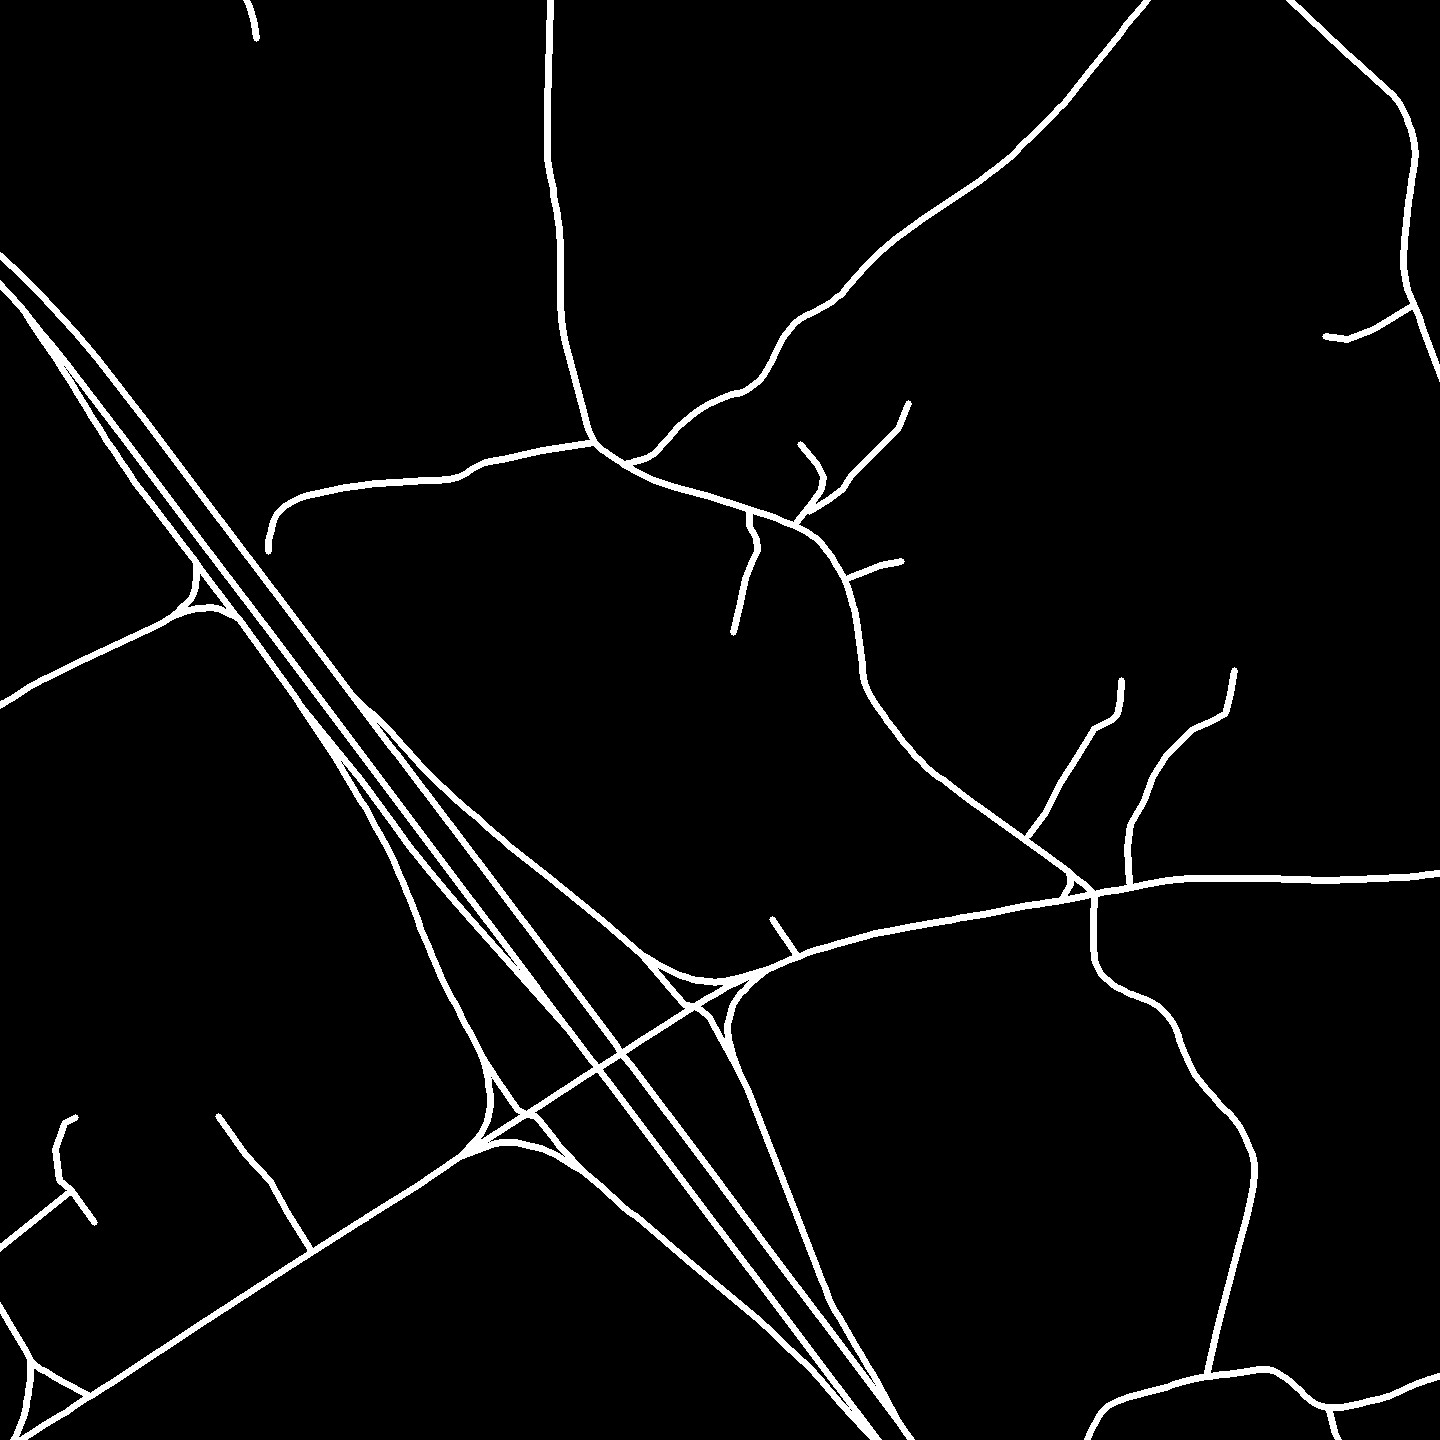
\includegraphics[width=\textwidth]{figs/E6/E6-label.jpg}
\caption{Label image.} \label{fig:E6_label_iamge}
\vspace{0.5cm} % separation vertically between the subfigures
\end{subfigure}
\hspace*{\fill} % separation between the subfigures
\begin{subfigure}{0.48\textwidth}
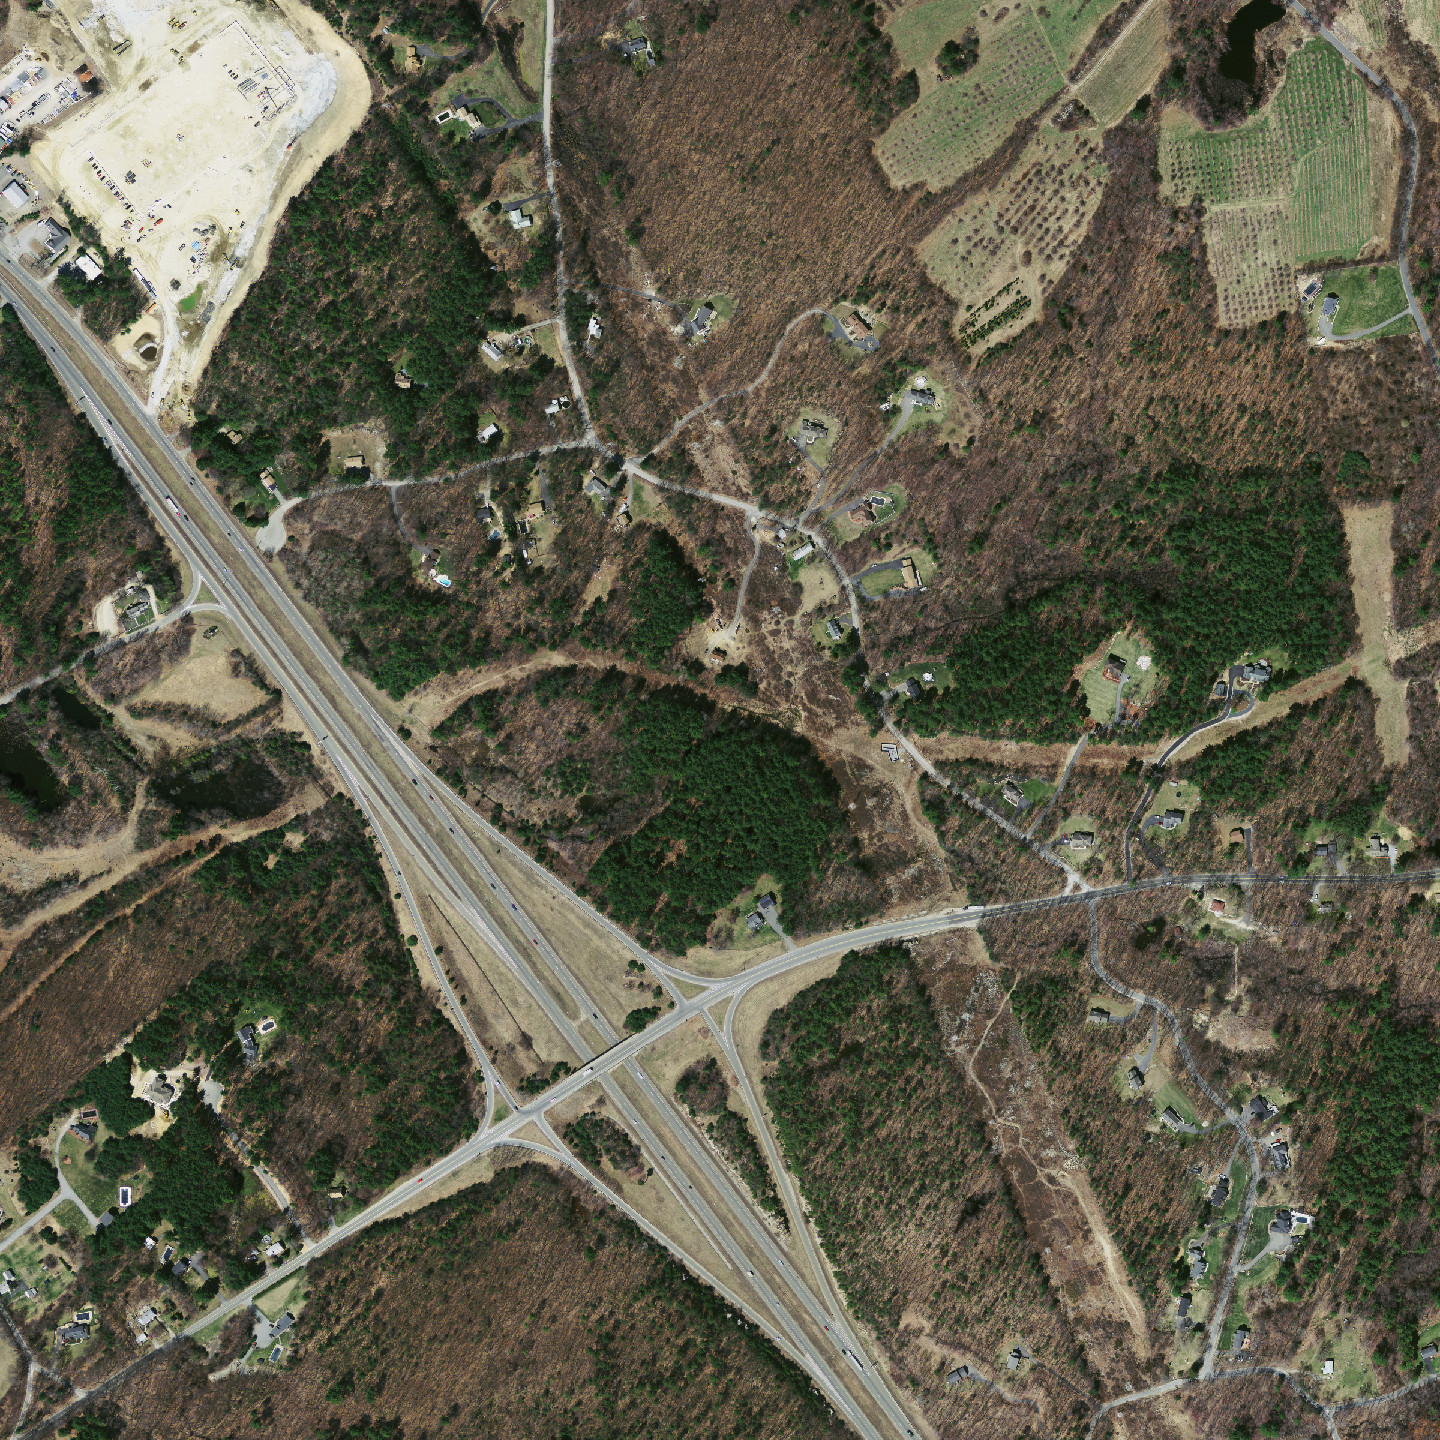
\includegraphics[width=\textwidth]{figs/E6/E6-image.jpg}
\caption{Aerial image.} \label{fig:E6_aerial_image}
\vspace{0.5cm} % separation vertically between the subfigures
\end{subfigure}

\begin{subfigure}{0.48\textwidth}
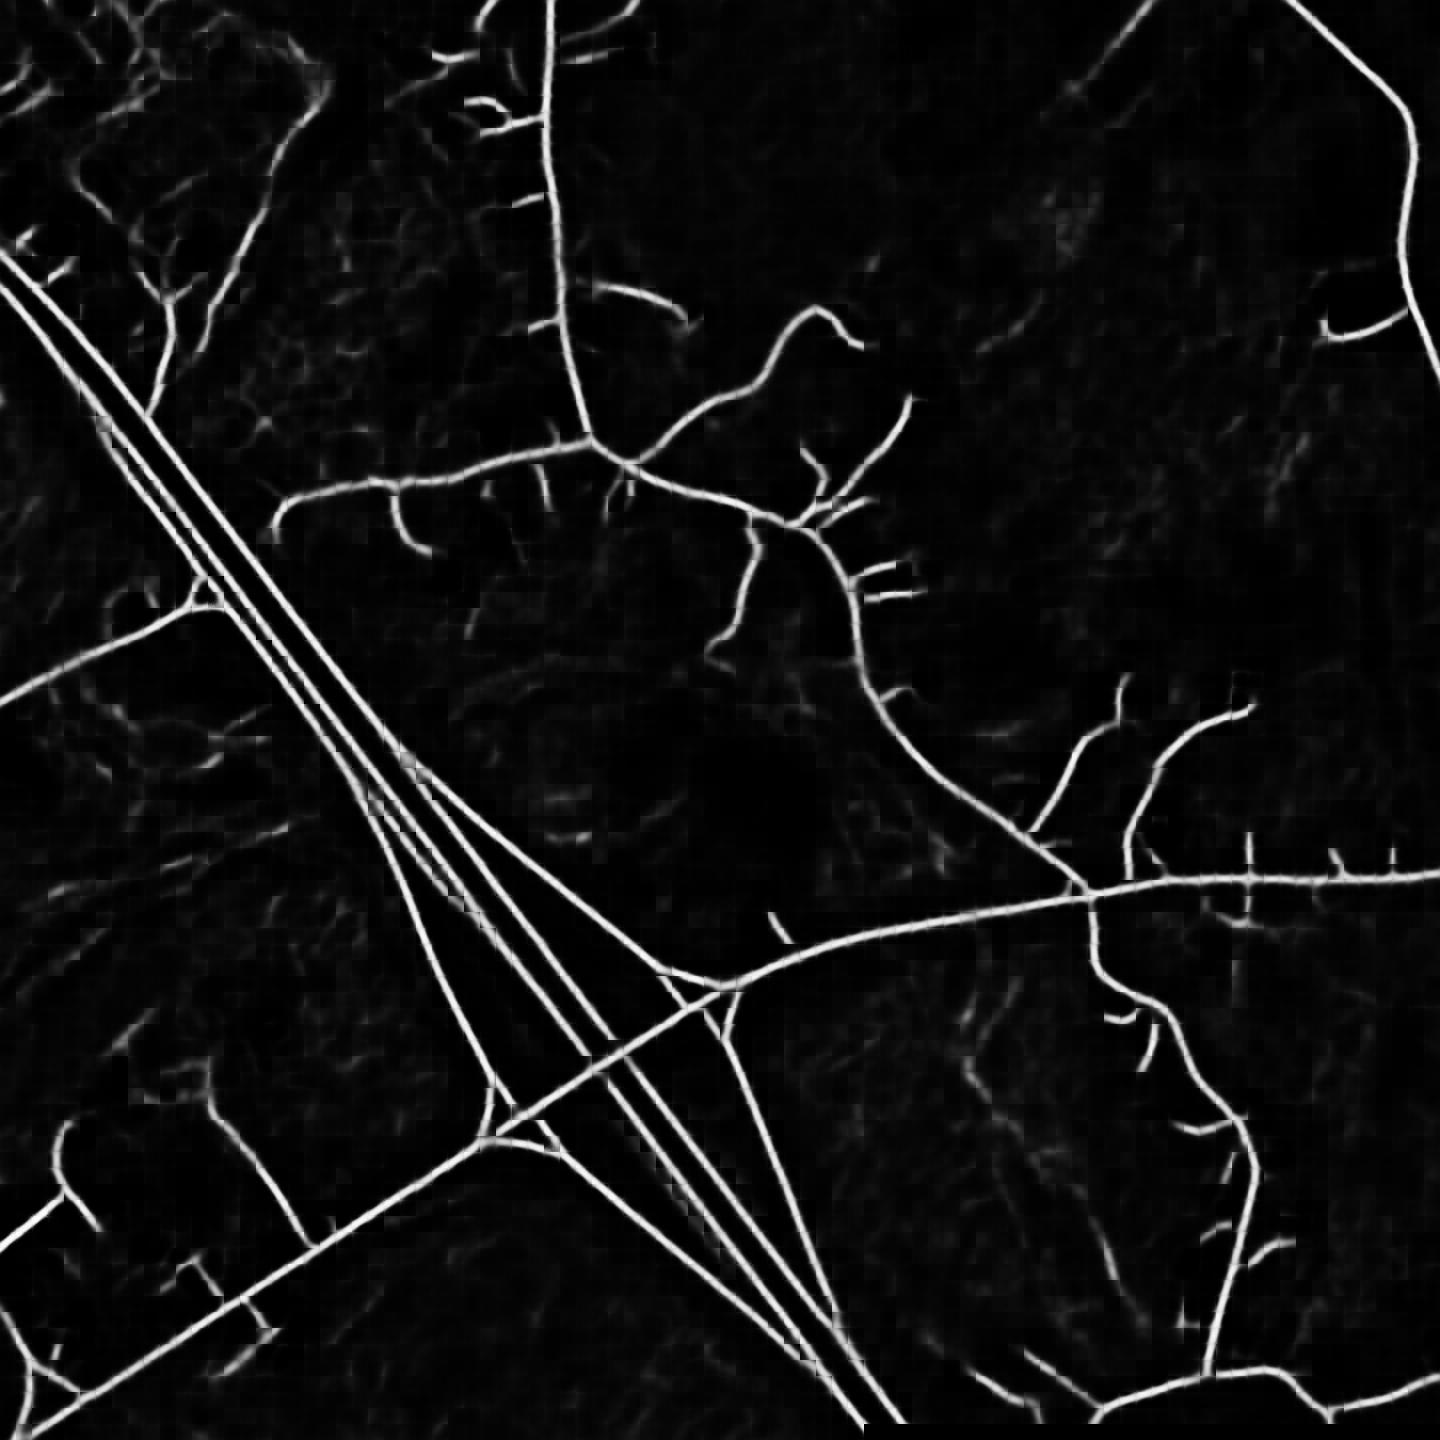
\includegraphics[width=\textwidth]{figs/E6/E6-pred.jpg}
\caption{Model predictions.} \label{fig:E6_model_predictions}
\end{subfigure}
\hspace*{\fill} % separation between the subfigures
\begin{subfigure}{0.48\textwidth}
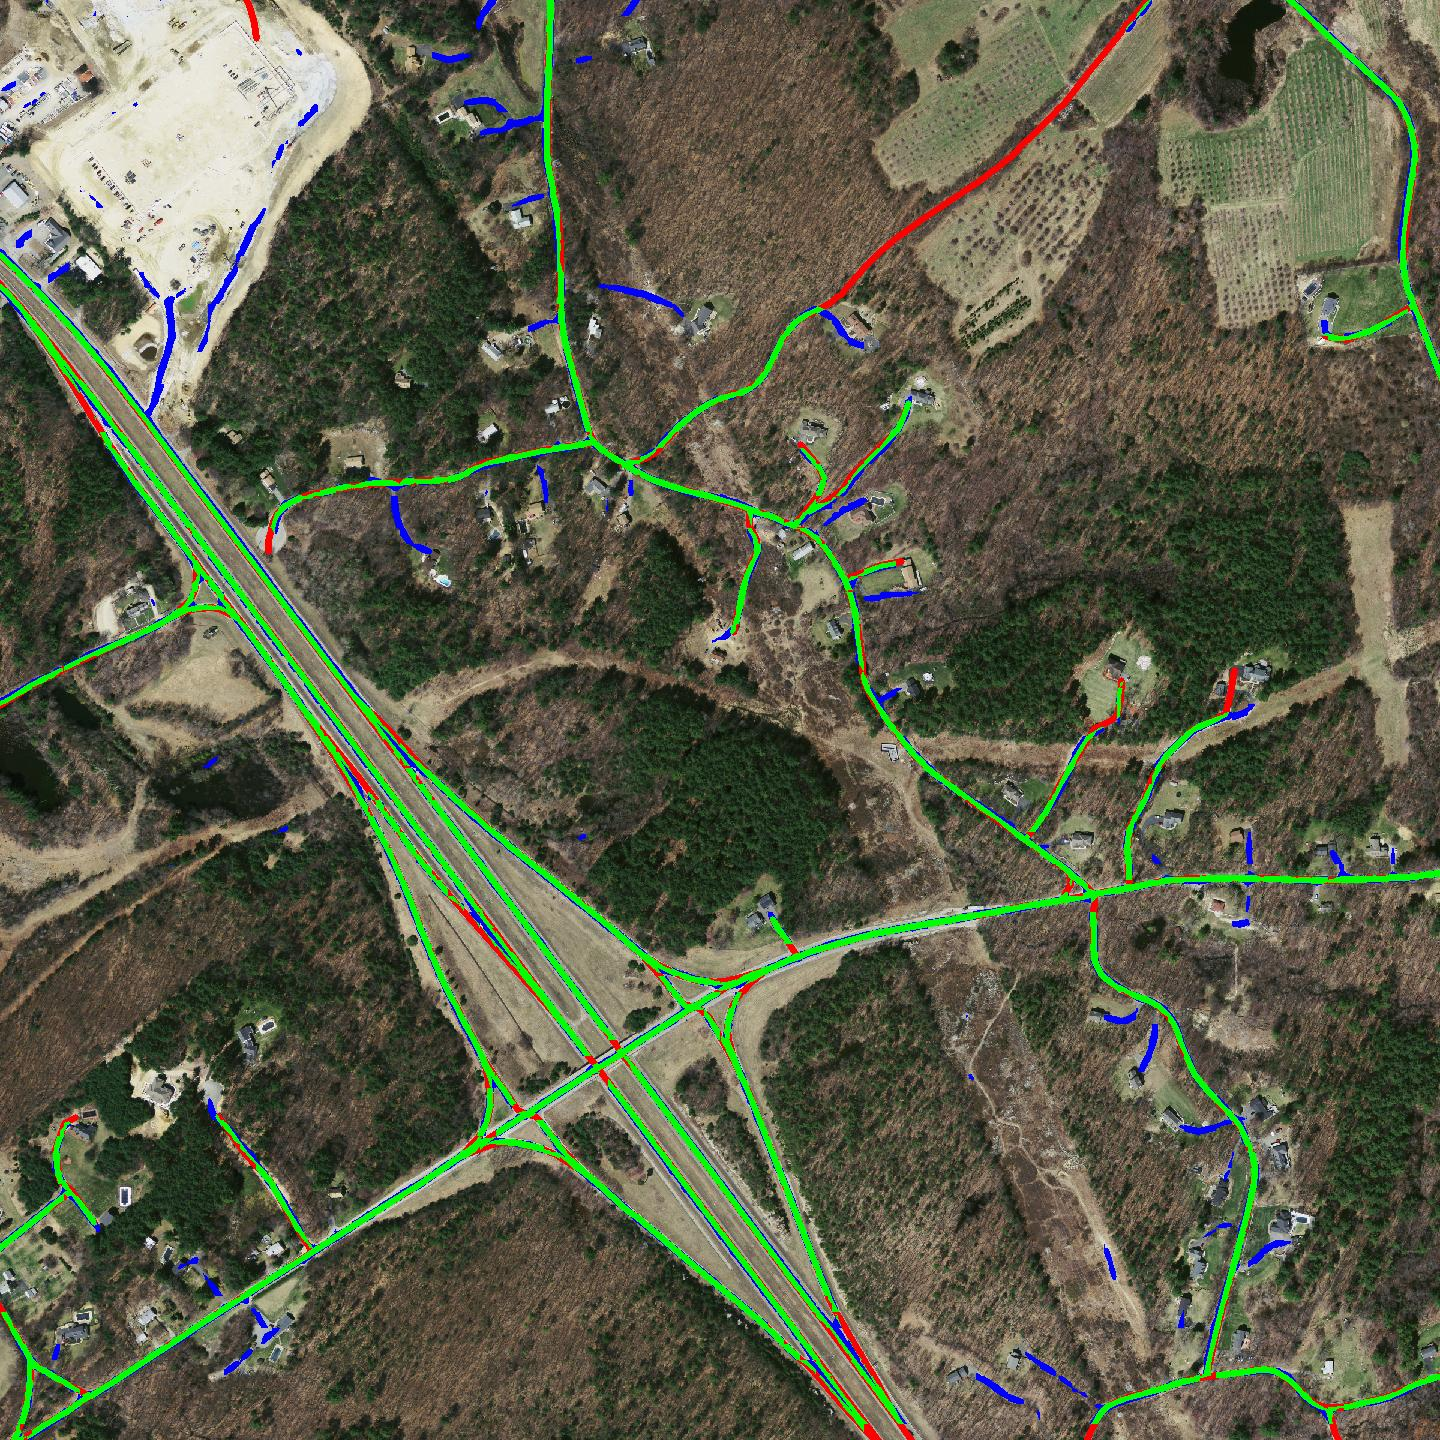
\includegraphics[width=\textwidth]{figs/E6/E6-hit.jpg}
\caption{Prediction hit and miss image.} \label{fig:E6_hit_image}
\end{subfigure}
\caption{E6 - Example of model's road detection performance. The aerial image is part of the test set in Massachusetts Roads Dataset} \label{fig:E6_performance}
\end{figure}

\todo[inline]{Mention limited amount of data. Curriculum learning advantageous for even bigger patch datasets?}
